\documentclass[tikz,border=4pt]{standalone}
% Shared visual grammar: role fills, dark connectors, and 7-point typography.
% Build each standalone figure from this directory. No external images required.
\pdfinfoomitdate=1
\pdftrailerid{}
\usepackage[T1]{fontenc}
\usepackage{helvet}
\renewcommand{\familydefault}{\sfdefault}
\usepackage{amsmath,amssymb}
\hyphenpenalty=10000
\exhyphenpenalty=10000
\usetikzlibrary{arrows.meta,calc,fit,positioning,decorations.pathreplacing,backgrounds}
\definecolor{ink}{HTML}{172B3A}
\definecolor{muted}{HTML}{586D85}
\definecolor{datafill}{HTML}{F1F5F9}
\definecolor{dataline}{HTML}{62748E}
\definecolor{modelfill}{HTML}{E5E9FF}
\definecolor{modelline}{HTML}{7887C7}
\definecolor{llmfill}{HTML}{FFE4E8}
\definecolor{llmline}{HTML}{E68494}
\definecolor{truthfill}{HTML}{D0FAE5}
\definecolor{truthline}{HTML}{35A782}
\newcommand{\seven}{\fontsize{7}{8.5}\selectfont}
\tikzset{
 every node/.append style={font=\seven,text=ink,align=center},
 box/.style={draw=dataline,fill=white,rounded corners=3pt,line width=.65pt,inner sep=5pt,minimum height=8mm},
 data/.style={box,fill=datafill},
 model/.style={box,draw=modelline,fill=modelfill},
 llm/.style={box,draw=llmline,fill=llmfill},
 truth/.style={box,draw=truthline,fill=truthfill},
 title/.style={font=\seven\bfseries,inner sep=1pt},
 word/.style={text=muted,inner sep=1pt,align=center},
 label/.style={fill=white,inner xsep=2pt,inner ysep=1pt,text=muted},
 flow/.style={-{Stealth[length=2.4mm,width=1.9mm]},draw=ink,line width=1.2pt,shorten >=1.5pt},
 branch/.style={-{Stealth[length=2mm,width=1.6mm]},draw=ink,line width=.9pt,shorten >=1pt},
 route/.style={draw=ink,line width=1.2pt},
 update/.style={-{Stealth[length=2.2mm,width=1.7mm]},draw=modelline,line width=1pt,dash pattern=on 3pt off 2pt,shorten >=1.5pt},
 boundary/.style={draw=dataline,dash pattern=on 3pt off 2pt,rounded corners=3pt,line width=.6pt},
 chip/.style={minimum height=4mm,inner xsep=3pt,inner ysep=1.5pt,rounded corners=2pt},
}
% Optional role key. Anchor at the center of an uncluttered final row.
\newcommand{\rolekey}[2]{
 \node[word,anchor=east] at (#1-6.6,#2) {\textit{Key}};
 \node[data,chip] at (#1-5.2,#2) {records / data};
 \node[model,chip] at (#1-1.9,#2) {learned model / policy};
 \node[llm,chip] at (#1+1.65,#2) {LLM signal};
 \node[truth,chip] at (#1+4.95,#2) {labels / evaluation};
}

\begin{document}
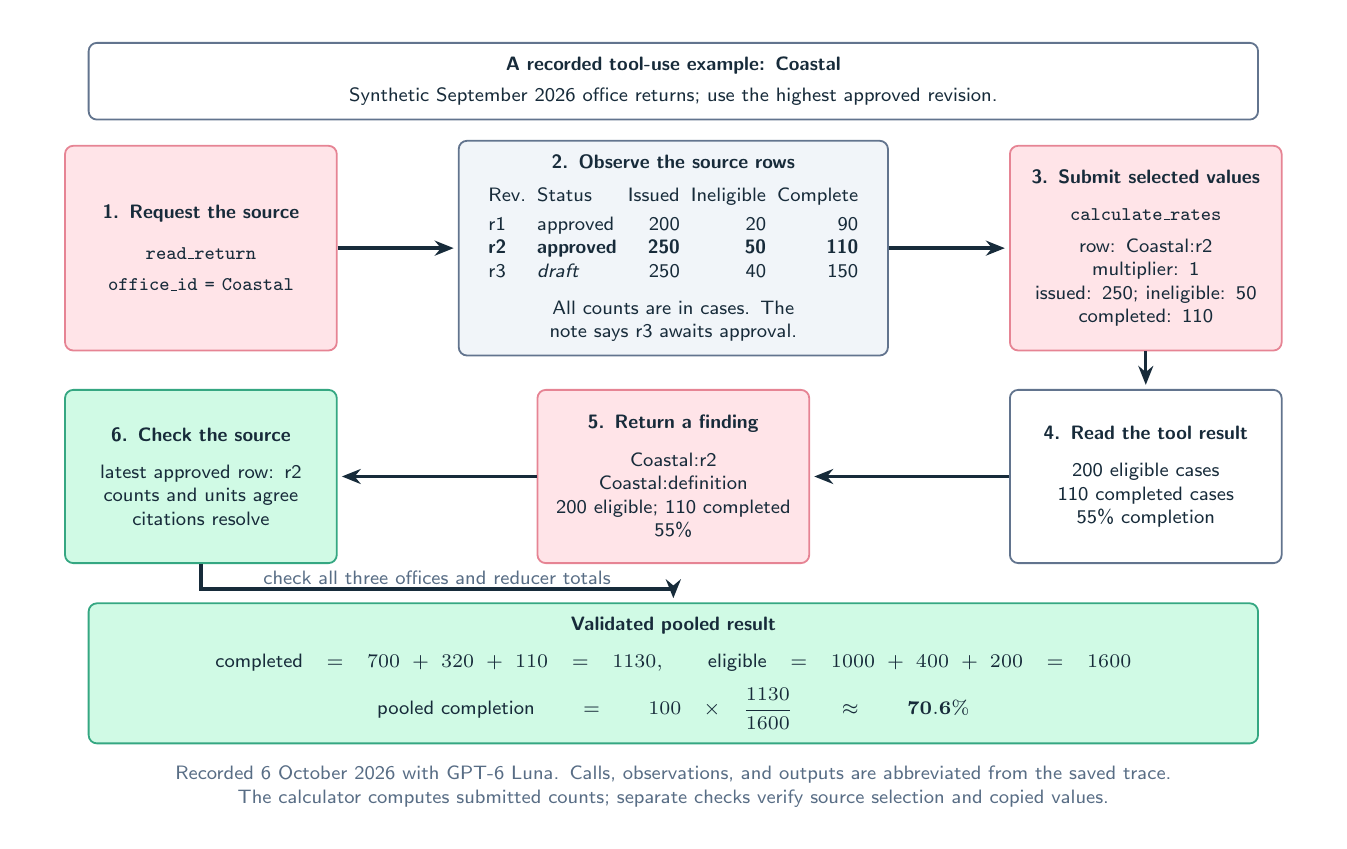
\begin{tikzpicture}

\useasboundingbox (-.2,.3) rectangle (16.2,-9.77);
\node[box,text width=145mm,minimum height=8mm] at (8,-.38) {\textbf{A recorded tool-use example: Coastal}\\[3pt]Synthetic September 2026 office returns; use the highest approved revision.};

\node[llm,text width=31mm,minimum height=26mm] (read) at (2,-2.5) {\textbf{1. Request the source}\\[6pt]\texttt{read\_return}\\[3pt]\texttt{office\_id = Coastal}};
\node[data,text width=51mm,minimum height=26mm] (source) at (8,-2.5) {\textbf{2. Observe the source rows}\\[5pt]
  \setlength{\tabcolsep}{2pt}
  \begin{tabular}{@{}llrrr@{}}
  Rev. & Status & Issued & Ineligible & Complete\\[2pt]
  r1 & approved & 200 & 20 & 90\\
  \textbf{r2} & \textbf{approved} & \textbf{250} & \textbf{50} & \textbf{110}\\
  r3 & \textit{draft} & 250 & 40 & 150
  \end{tabular}\\[5pt]
  All counts are in cases. The note says r3 awaits approval.};
\node[llm,text width=31mm,minimum height=26mm] (compute) at (14,-2.5) {\textbf{3. Submit selected values}\\[5pt]\texttt{calculate\_rates}\\[3pt]row: Coastal:r2\\multiplier: 1\\issued: 250; ineligible: 50\\completed: 110};
\draw[flow] (read) -- (source);
\draw[flow] (source) -- (compute);

\node[box,text width=31mm,minimum height=22mm] (observed) at (14,-5.4) {\textbf{4. Read the tool result}\\[5pt]200 eligible cases\\110 completed cases\\55\% completion};
\node[llm,text width=31mm,minimum height=22mm] (finding) at (8,-5.4) {\textbf{5. Return a finding}\\[5pt]Coastal:r2\\Coastal:definition\\200 eligible; 110 completed\\55\%};
\node[truth,text width=31mm,minimum height=22mm] (check) at (2,-5.4) {\textbf{6. Check the source}\\[5pt]latest approved row: r2\\counts and units agree\\citations resolve};
\draw[flow] (compute) -- (observed);
\draw[flow] (observed) -- (finding);
\draw[flow] (finding) -- (check);

\node[truth,text width=145mm,minimum height=16mm] (pooled) at (8,-7.9) {\textbf{Validated pooled result}\\[5pt]
  $\text{completed}=700+320+110=1130,\qquad\text{eligible}=1000+400+200=1600$\\[5pt]
  $\text{pooled completion}=100\times\dfrac{1130}{1600}\approx\mathbf{70.6\%}$};
\draw[flow] (check.south) -- (2,-6.83) -- node[label,above] {check all three offices and reducer totals} (8,-6.83) -- (pooled.north);

\node[word,text width=145mm] at (8,-9.34) {Recorded 6 October 2026 with GPT-6 Luna. Calls, observations, and outputs are abbreviated from the saved trace.\\The calculator computes submitted counts; separate checks verify source selection and copied values.};

\end{tikzpicture}
\end{document}
